% ==============================================================================================
\chapter{Static uniform load on circular area on a 3D elastic halfspace} \label{ch:boussinesq}
% ==============================================================================================

% ----------------------------------------------------------------------------------------------
\section{Introduction}
% ----------------------------------------------------------------------------------------------
This benchmark compares the STEM numerical solution with the analytical solution for a static, uniformly
distributed circular load applied to the surface of an elastic half-space, which is discretised using
symmetry about the x-y and y-z planes.

The analytical solution is presented in~\cite[Chapter 13.124]{Timoshenko_1951}.
It provides closed-form expressions for the vertical stress beneath the centre of the circular load and for the vertical
displacement along the surface of the elastic half-space, enabling direct comparison with the numerical model.

% ----------------------------------------------------------------------------------------------
\section{Model Description}
% ----------------------------------------------------------------------------------------------

% ..............................................................................................
\subsection{Geometry, mesh and loading}
% ..............................................................................................
The soil domain is modelled in 3D and  represents a \qty{10}{\meter} $\times$ \qty{30}{\meter}
$\times$ \qty{10}{\meter} soil layer, modelled with second-order tetrahedral elements. The mesh uses an average
element size of \qty{1}{\meter}.
Figure~\ref{fig:boussinesq_mesh} illustrates the geometry and mesh adopted for the analysis.

A quarter circular distributed load, consistent with the applied symmetry conditions, is applied at the surface with
a radius of \qty{0.1}{\meter}. A downward surface load with magnitude \qty{10}{\kilo\newton\per\meter\squared} is applied.
The mesh is locally refined beneath the loaded area, with an average element size of \qty{0.015}{\meter}.

The nodes at the bottom are fully fixed, while the four vertical sides are restrained only in the normal direction
(roller boundaries) to allow vertical and tangential movement.

\begin{figure}
    \centering
    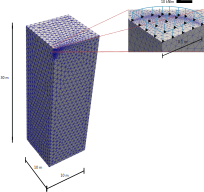
\includegraphics[width=0.75\textwidth]{boussinesq/boussinesq.pdf}
    \caption{Geometry and mesh adopted for the benchmark with a circular distributed load.}
    \label{fig:boussinesq_mesh}
\end{figure}

% ..............................................................................................
\subsection{Materials and numerical parameters}
% ..............................................................................................
The soil is modelled as a one-phase continuum with a linear elastic constitutive law, with the
following parameters:

\begin{itemize}[noitemsep,topsep=0pt,parsep=0pt,partopsep=0pt]
    \item Young's modulus: \qty{20}{\mega\pascal},
    \item Poisson ratio: \qty{0.3}{},
    \item Density: \qty{2000}{\kilogram\per\meter\cubed}.
\end{itemize}


% ----------------------------------------------------------------------------------------------
\section{Results}
% ----------------------------------------------------------------------------------------------
Figure~\ref{fig:boussinesq_results} presents the vertical displacement along the surface of the elastic half-space,
and the vertical stress below the centre of the circular load.
The figure compares the STEM results against the analytical solution.
If follows that there is an agreement between both solutions, demonstrating the accuracy of STEM
for this type of static loading condition.

\begin{figure}[h]
    \centering
    \includegraphics[width=0.8\textwidth]{boussinesq/boussinesq_comparison.pdf}
    \caption{(a) Vertical displacement along the surface of the half-space, (b) vertical stress below the centre of the
    circular load.}
    \label{fig:boussinesq_results}
\end{figure}
